\def\duedate{10/13/22}
\def\HWnum{5}
% Document setup
\documentclass[12pt]{article}
\usepackage[margin=1in]{geometry}
\usepackage{fancyhdr}
\usepackage{lastpage}

\pagestyle{fancy}
\lhead{Richard Whitehill}
\chead{MATH 757 -- HW \HWnum}
\rhead{\duedate}
\cfoot{\thepage \hspace{1pt} of \pageref{LastPage}}

% Encoding
\usepackage[utf8]{inputenc}
\usepackage[T1]{fontenc}

% Math/Physics Packages
\usepackage{amsmath}
\usepackage{amssymb}
\usepackage{mathtools}
\usepackage[arrowdel]{physics}
\usepackage{siunitx}

\AtBeginDocument{\RenewCommandCopy\qty\SI}

% Reference Style
\usepackage{hyperref}
\hypersetup{
    colorlinks=true,
    linkcolor=blue,
    filecolor=magenta,
    urlcolor=cyan,
    citecolor=green
}

\newcommand{\eref}[1]{Eq.~(\ref{eq:#1})}
\newcommand{\erefs}[2]{Eqs.~(\ref{eq:#1})--(\ref{eq:#2})}

\newcommand{\fref}[1]{Fig.~\ref{fig:#1}}
\newcommand{\frefs}[2]{Figs.~\ref{fig:#1}--\ref{fig:#2}}

\newcommand{\tref}[1]{Table~\ref{tab:#1}}
\newcommand{\trefs}[2]{Tables~\ref{tab:#1}-\ref{tab:#2}}

% Figures and Tables 
\usepackage{graphicx}
\usepackage{float}

\newcommand{\bef}{\begin{figure}[h!]\begin{center}}
\newcommand{\eef}{\end{center}\end{figure}}

\newcommand{\bet}{\begin{table}[h!]\begin{center}}
\newcommand{\eet}{\end{center}\end{table}}

% tikz
\usepackage{tikz}
\usetikzlibrary{calc}
\usetikzlibrary{decorations.pathmorphing}
\usetikzlibrary{decorations.markings}
\usetikzlibrary{arrows.meta}
\usetikzlibrary{positioning}

% tcolorbox
\usepackage[most]{tcolorbox}
\usepackage{xcolor}
\usepackage{xifthen}
\usepackage{parskip}

\newcommand*{\eqbox}{\tcboxmath[
    enhanced,
    colback=black!10!white,
    colframe=black,
    sharp corners,
    size=fbox,
    boxsep=8pt,
    boxrule=1pt
]}

% Miscellaneous Definitions/Settings
\newcommand{\prob}[2]{\textbf{#1)} #2}
\newcommand{\reals}{\mathbb{R}}
\newcommand{\integers}{\mathbb{Z}}
\newcommand{\naturals}{\mathbb{N}}
\newcommand{\rationals}{\mathbb{Q}}
\newcommand{\complexs}{\mathbb{C}}

\setlength{\parskip}{\baselineskip}
\setlength{\parindent}{0pt}
\setlength{\headheight}{14.49998pt}
\addtolength{\topmargin}{-2.49998pt}







\begin{document}
    

\prob{4.2.2}{
Consider the equation $u_{tt} = c^2 u_{xx}$ for $0 < x < l$, with the boundary conditions $u_{x}(0,t) = 0$, $u(l,t) = 0$ (Neumann at the left, Dirichlet at the right).
}

a) Show that the eigenfunctions are $\cos{\big[ \big( n+\frac{1}{2} \big) \pi x / l \big]}$

We want to solve the equation $u_{tt} - Au = 0$, where the linear operator $A = -c^2\partial_{x}^2$.
Hence, the eigenequation for the operator $A$ is 
\begin{eqnarray}
    \label{eq:eigeneq}
    -c^2 \pdv[2]{f}{x} = \lambda f(x) \Leftrightarrow \pdv[2]{f}{x} + \frac{\lambda}{c^2}f(x) = 0
,\end{eqnarray}
which has solution $f(x) = C_1 \cos{(\omega x)} + C_{2} \sin{(\omega x)}$, where $\lambda = \omega^2 c^2$.
Now, we plug in our boundary conditions:
\begin{align}
    \label{eq:solve-C2}
    \pdv{f}{x} = C_{1}\omega \sin{(\omega x)} - C_{2}\omega\cos{(\omega x)} = 0 \Rightarrow C_{2} = 0 \\
    f(l) = C_1 \cos{(\omega l)} = 0
.\end{align}
Now, $f(x) \not\equiv 0$, so we can satisfy the latter equation of the two above by imposing
\begin{eqnarray}
    \label{eq:solve-omega}
    \omega l = \frac{(2n+1)\pi}{2} \Leftrightarrow \omega = \frac{\big(n + \frac{1}{2}\big)\pi}{l}
,\end{eqnarray}
where $n \in \naturals$ (note: $\lambda > 0$ for $\partial_{x}^2$).
Hence, our eigenfunctions of $A$ are just
\begin{eqnarray}
    \label{eq:eigenfuncs}
    \eqbox{
    f_{n}(x) = \cos{\big[ \big(n+\frac{1}{2}\big)\pi x / l \big]}
}
,\end{eqnarray}
where we dropped the coefficient since scaling the eigenfunction also produces a valid eigenfunction (albeit not a linearly independent one!).

b) Write the series expansion for a solution $u(x,t)$.

Observe that the equation $u_{tt} - Au = 0$ has solution $u(t) = C_1 \cos{(\sqrt{A} t)} + C_2 \sin{(\sqrt{A} t)}$ and $g(A)f_{n}(x) = g(\lambda)f_{n}(x)$, assuming that $g$ is a function with a valid, convergent Taylor expansion, which both $\sin{x}$ and $\cos{x}$ do.
Hence, our solution
\begin{eqnarray}
    \label{eq:solution-general}
    \eqbox{
    u(x,t) = \sum_{n \in \naturals} \big[ C_{1,n} \cos{(\omega_{n}c t)} + C_{2,n} \sin{(\omega_{n} ct)} \big] f_{n}(x)
}
,\end{eqnarray}
where $\omega_{n}$ is given by \eref{solve-omega} and $f_{n}(x)$ is given by \eref{eigenfuncs}.


\prob{4.2.3}{
    Solve the Schr\"{o}dinger equation $u_{t} = ik u_{xx}$ for real $k$ in the interval $0 < x < l$ with the boundary conditions $u_{x}(0,t) = 0$, $u(l,t) = 0$.
}

Schr\"{o}dinger's equation reads $u_{t} + ikAu = 0$, where the linear operator $A = -\partial^2_{x}$.
This equation has the simple solution $u = \exp(-i\frac{t}{k}A)$, and the operator $A$ has eigenfunction $f(x) = C_{1} \cos{\sqrt{\lambda} x} + C_{2} \sin{\sqrt{\lambda} x}$
From the boundary conditions, we find that $C_{1} = 0$ and $\sqrt{\lambda_{n}} = (n+\frac{1}{2})\pi/l$ ($n \in \naturals$), as in the previous problem.
The general solution to the Schr\"{o}dinger equation for the boundary conditions in this problem is given as
\begin{eqnarray}
    \label{eq:solution-Schrodinger}
    \eqbox{
    u(x,t) = \sum_{n \in \naturals} e^{-i\frac{t}{k}A} C_{n}\cos{\sqrt{\lambda_{n}}x} = \sum_{n \in \naturals} C_{n} e^{-i\lambda_{n}t/k} \cos{\sqrt{\lambda_{n}} x}
}
,\end{eqnarray}
where $\lambda_{n} = (n+\frac{1}{2})^2\pi^2/l^2$.

\prob{5.1.2}{
Let $\phi(x) \equiv x^2$ for $0 \leq x \leq 1 = l$.
}

a) Calculate its Fourier sine series.

We write
\begin{eqnarray}
    \label{eq:sine-series}
    x^2 = \sum_{n=1}^{\infty} A_{n} \sin{(n\pi x)} 
,\end{eqnarray}
in the interval $[0,1]$, where
\begin{eqnarray}
    \label{eq:coeff-sine}
    A_{n} = 2 \int_{0}^{1} x^2 \sin{(n \pi x)} \dd{x} = \frac{2[(2 - \pi^2n^2)(-1)^{n} - 2]}{\pi^3 n^3} = 
    \begin{cases}
        -\frac{1}{\pi n}, & n \equiv 0 \mod{2} \\
        \frac{\pi^2n^2 - 4}{\pi^3 n^3}, & n \equiv 1 \mod{2}
    \end{cases}
.\end{eqnarray}
Hence,
\begin{align}
    \label{eq:sine-series-with-coeff}
    \eqbox{
    x^2 = \sum_{n=1}^{\infty} \frac{2(2-\pi^2n^2)(-1)^{n} - 4}{\pi^3n^3} \sin{(n\pi x)}
}
.\end{align}
Interestingly, this sequence converges point-wise to $x^2$ everywhere except $x=1$, to which it converges to $0$ trivially.

\begin{figure}[H]
\begin{center}
    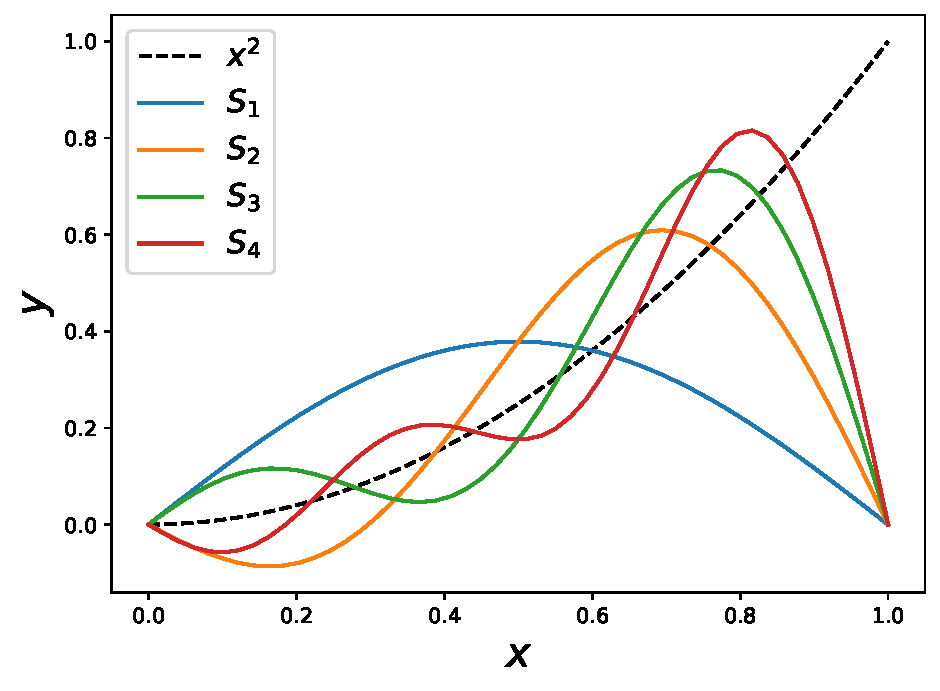
\includegraphics[width=0.75\textwidth]{./prob5_1_2a.pdf}
\end{center} 
\caption{
Plot of $x^2$ and partial sums of Fourier sine series $S_{N} = \sum_{n=1}^{N} A_{n}\sin{(n\pi x)}$.
}
\label{fig:partial-sums-sine-series}
\end{figure}

b) Calculate its Fourier cosine series.

The cosine series is
\begin{eqnarray}
    \label{eq:cosine-series}
    x^2 = \frac{A_0}{2} + \sum_{n=1}^{\infty} A_{n}\cos{(n\pi x)}
,\end{eqnarray}
where
\begin{eqnarray}
    \label{eq:A0-cosine}
    A_{0} = 2 \int_{0}^{1} x^2 \dd{x} = \frac{2}{3}
\end{eqnarray}
and
\begin{eqnarray}
    \label{eq:An-cosine}
    A_{n} = 2 \int_{0}^{1} x^2 \cos{(n\pi x)} = \frac{2(-1)^{n}}{\pi^2n^2}
.\end{eqnarray}
This gives us the sum
\begin{align}
    \label{eq:x2-cosine-series}
    \eqbox{
    x^2 = \frac{1}{3} + \sum_{n=1}^{\infty} \frac{2(-1)^{n}}{\pi^2 n^2} \cos{(n \pi x)}
}
.\end{align}

\begin{figure}[H]
\begin{center}
    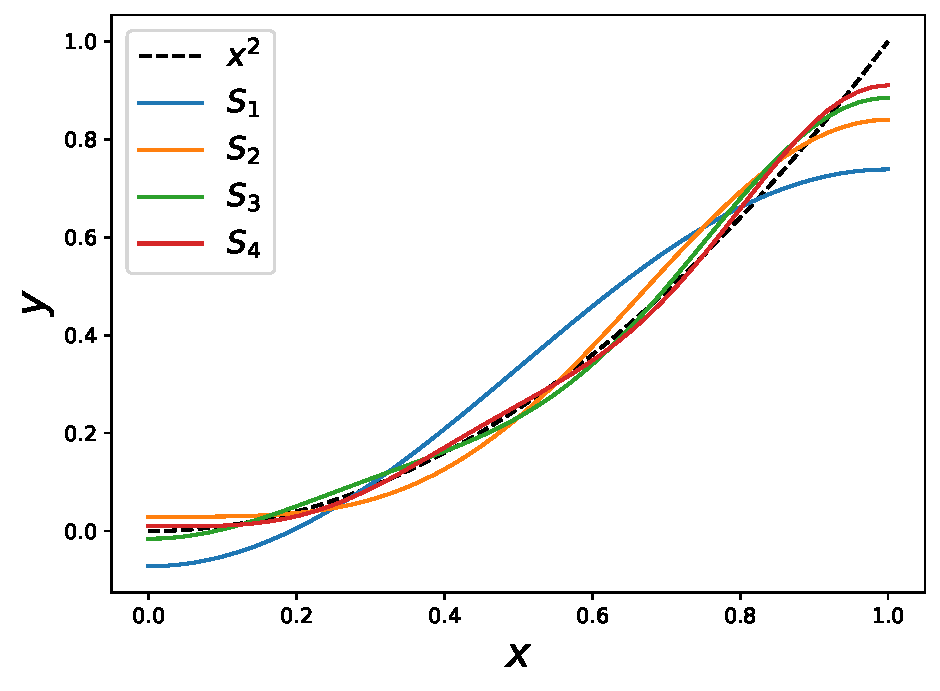
\includegraphics[width=0.75\textwidth]{./prob5_1_2b.pdf}
\end{center} 
\caption{
Plot of $x^2$ and partial sums of Fourier cosine series $S_{N} = \frac{1}{3} + \sum_{n=1}^{N} A_{n}\cos{(n\pi x)}$.
}
\label{fig:partial-sums-cosine-series}

\end{figure}


\prob{5.1.4}{
Find the Fourier cosine series of the function $|\sin{x}|$ in the interval $(-\pi,\pi)$.
Use it to find the sums
\begin{eqnarray}
\label{eq:goal-sums}
    \sum_{n=1}^{\infty} \frac{1}{4n^2 - 1} \quad {\rm and} \quad \sum_{n=1}^{\infty} \frac{(-1)^{n}}{4n^2 - 1}
.\end{eqnarray} 
}

Observe that $\sin{x} > 0$ for $x \in [0,\pi]$, so we can write
\begin{eqnarray}
    \label{eq:cosine-series-4}
    \sin{x} = \frac{A_0}{2} + \sum_{n=1}^{\infty} A_{n}\cos{n x}
,\end{eqnarray}
where 
\begin{eqnarray}
    \label{eq:A0-coeff-4}
    A_0 = \frac{2}{\pi} \int_{0}^{\pi} \sin{x} \dd{x} = \frac{4}{\pi} 
\end{eqnarray}
and
\begin{eqnarray}
    \label{eq:An-coeff-4}
    A_{n} = \frac{2}{\pi} \int_{0}^{\pi} \sin{x} \cos{nx} \dd{x} = \frac{2[1 - (-1)^{n}]}{\pi(1 - n^2)} = 
    \begin{cases}
        0, & n \equiv 1 \mod{2} \\
        -\frac{4}{\pi(n^2 - 1)}, & n \equiv 0 \mod{2}
    \end{cases}
.\end{eqnarray}
Hence,
\begin{eqnarray}
    \label{eq:sine-fourier}
    \sin{x} = \frac{4}{\pi}\Bigg[ \frac{1}{2} - \sum_{n=1}^{\infty} \frac{\cos{2nx}}{4n^2 - 1} \Bigg]
.\end{eqnarray}
Actually, this is the expansion for $|\sin{x}|$ on $(-\pi,\pi)$ since it is an even function and $\cos$ is even.
We can then say at $x = 0$
\begin{eqnarray}
    \label{eq:sum1}
    \eqbox{
    \sum_{n=1}^{\infty} \frac{1}{4n^2-1} = \frac{1}{2}
}
.\end{eqnarray}
Next, if we set $x = \pi/2$
\begin{eqnarray}
    \label{eq:sum2}
    1 = \frac{4}{\pi}\Bigg[ \frac{1}{2} - \sum_{n=1}^{\infty} \frac{(-1)^{n}}{4n^2 - 1} \Bigg] 
,\end{eqnarray}
and rearranging gives
\begin{eqnarray}
    \label{eq:sum2-sol}
    \eqbox{
    \sum_{n=1}^{\infty} \frac{(-1)^{n}}{4n^2 - 1} = \frac{1}{2} - \frac{\pi}{4} = \frac{2 - \pi}{4}
}
.\end{eqnarray}







\end{document}
